\begin{maintask}{E}
  \subsection*{課題内容}
  学外のWebサイトにwgetでHTTP/HTTPSアクセスし，通信の手順（ゲートウェイのMACアドレス解決，DNS，HTTP，HTTPS）を確認した．

  \subsection*{実験方法}
  \begin{enumerate}
    \item 経路表と近隣キャッシュを記録
      \begin{minted}{zsh}
        ip -4 route
        ip -6 route
        ip ne
      \end{minted}

    \item 以下のサイトごとに，キャプチャ開始，wget実行，キャプチャ停止を繰り返す（pcapはサイトごとに分ける）．tcpdumpとwgetは別のターミナルで実行し，wgetの終了後にCtrl-Cでキャプチャを止める．
      \begin{minted}{zsh}
        (IPv4のみ)    tcpdump -i eth1 -s 0 -w day2_E_sapporo.pcap 'not port 4200'
                      wget www.city.sapporo.jp
        (IPv4/IPv6)   tcpdump -i eth1 -s 0 -w day2_E_hokkaido.pcap 'not port 4200'
                      wget www.pref.hokkaido.lg.jp
        (IPv6のみ指定) tcpdump -i eth1 -s 0 -w day2_E_keio.pcap 'not port 4200'
                      wget www.keio.ac.jp
      \end{minted}
      % TODO: keioは「IPv6のみ指定」。実際に -6 を付けたならここも wget -6 www.keio.ac.jp に直す

    \item 各pcapをWiresharkで開き，次のフィルタを適用
      \begin{minted}{text}
        (arp || icmpv6.type == 135 || icmpv6.type == 136 || dns || tcp.port == 80 || tcp.port == 443) && !(dns.qry.type == 12)
      \end{minted}
  \end{enumerate}

  \subsection*{結果}
  実行前の経路表と近隣キャッシュを出力\ref{out:route_e}に，サイトごとのtcpdumpとwgetの実行結果を
  出力\ref{out:e_sapporo}，
  出力\ref{out:e_hokkaido}，
  出力\ref{out:e_keio}
  に示した．

  \begin{termout}[H]
    \caption{実行前の経路表と近隣キャッシュ}\label{out:route_e}
    \begin{minted}{zsh}
    guest@host82:~$ ip -4 route
    default via 172.28.0.1 dev eth1                                                                          
    172.27.0.0/24 dev eth0 proto kernel scope link src 172.27.0.182                                          
    172.28.0.0/24 dev eth1 proto kernel scope link src 172.28.0.182                                          

    guest@host82:~$ ip -6 route                                                                              
    2001:2f8:40:11da::/64 dev eth1 proto kernel metric 256 pref medium                                       
    fe80::/64 dev eth1 proto kernel metric 256 pref medium                                                   
    default via 2001:2f8:40:11da::1 dev eth1 metric 1024 pref medium                                         

    guest@host82:~$ ip ne                                                                                    
    172.28.0.203 dev eth1 lladdr e6:aa:7d:51:5c:ed STALE                                                     
    172.28.0.1 dev eth1 lladdr a2:1e:33:b9:98:ef REACHABLE                                                   
    fe80::fc89:1ff:fec2:833a dev eth1 lladdr fe:89:01:c2:83:3a STALE                                         
    2001:2f8:40:11da::200 dev eth1 lladdr fe:89:01:c2:83:3a STALE                                            
    2001:2f8:40:11da::203 dev eth1 lladdr e6:aa:7d:51:5c:ed STALE                                            
    fe80::e4aa:7dff:fe51:5ced dev eth1 lladdr e6:aa:7d:51:5c:ed REACHABLE                                    
    fe80::a01e:33ff:feb9:98ef dev eth1 lladdr a2:1e:33:b9:98:ef router REACHABLE                             
    2001:2f8:40:11da::1 dev eth1 lladdr a2:1e:33:b9:98:ef router REACHABLE        
    \end{minted}
  \end{termout}

  \begin{termout}[H]
    \caption{www.city.sapporo.jp の tcpdump と wget の実行結果}\label{out:e_sapporo}
    \begin{minted}{zsh}
    guest@host82:~$ tcpdump -i eth1 -s 0 -w day2_E_sapporo.pcap 'not port 4200'
    tcpdump: listening on eth1, link-type EN10MB (Ethernet), capture size 262144 bytes
    ^C152 packets captured
    154 packets received by filter
    0 packets dropped by kernel

    guest@host82:~$ wget www.city.sapporo.jp
    --2026-11-10 00:55:19--  http://www.city.sapporo.jp/
    www.city.sapporo.jp (www.city.sapporo.jp) をDNSに問いあわせています... 45.60.112.77
    www.city.sapporo.jp (www.city.sapporo.jp)|45.60.112.77|:80 に接続しています... 接続しました。
    HTTP による接続要求を送信しました、応答を待っています... 301 Moved Permanently
    場所: https://www.city.sapporo.jp/ [続く]
    --2026-11-10 00:55:19--  https://www.city.sapporo.jp/
    www.city.sapporo.jp (www.city.sapporo.jp)|45.60.112.77|:443 に接続しています... 接続しました。
    HTTP による接続要求を送信しました、応答を待っています... 200 OK
    長さ: 38349 (37K) [text/html]
    `index.html' に保存中

    index.html                 100%[=====================================>]  37.45K  --.-KB/s    in 0.03s   

    2026-11-10 00:55:20 (1.27 MB/s) - `index.html' へ保存完了 [38349/38349]
    \end{minted}
  \end{termout}

  \begin{termout}[H]
    \caption{www.pref.hokkaido.lg.jp の tcpdump と wget の実行結果}\label{out:e_hokkaido}
    \begin{minted}{zsh}
    guest@host82:~$ tcpdump -i eth1 -s 0 -w day2_E_hokkaido.pcap 'not port 4200'
    tcpdump: listening on eth1, link-type EN10MB (Ethernet), capture size 262144 bytes
    ^C170 packets captured
    172 packets received by filter
    0 packets dropped by kernel

    guest@host82:~$ wget www.pref.hokkaido.lg.jp
    --2026-11-10 00:57:19--  http://www.pref.hokkaido.lg.jp/
    www.pref.hokkaido.lg.jp (www.pref.hokkaido.lg.jp) をDNSに問いあわせています... 2a02:e980:10e::4d, 45.60.112.77
    www.pref.hokkaido.lg.jp (www.pref.hokkaido.lg.jp)|2a02:e980:10e::4d|:80 に接続しています... 接続しました。
    HTTP による接続要求を送信しました、応答を待っています... 302 Found
    場所: https://www.pref.hokkaido.lg.jp/ [続く]
    --2026-11-10 00:57:19--  https://www.pref.hokkaido.lg.jp/
    www.pref.hokkaido.lg.jp (www.pref.hokkaido.lg.jp)|2a02:e980:10e::4d|:443 に接続しています... 接続しました。
    HTTP による接続要求を送信しました、応答を待っています... 200 OK
    長さ: 特定できません [text/html]
    `index.html.1' に保存中

    index.html.1                   [ <=>                                  ]  93.46K  --.-KB/s    in 0.07s   

    2026-11-10 00:57:20 (1.40 MB/s) - `index.html.1' へ保存終了 [95704]
    \end{minted}
  \end{termout}

  \begin{termout}[H]
    \caption{www.keio.ac.jp の tcpdump と wget の実行結果}\label{out:e_keio}
    \begin{minted}{zsh}
    guest@host82:~$ tcpdump -i eth1 -s 0 -w day2_E_keio.pcap 'not port 4200'
    tcpdump: listening on eth1, link-type EN10MB (Ethernet), capture size 262144 bytes
    ^C296 packets captured
    298 packets received by filter
    0 packets dropped by kernel

    guest@host82:~$ wget www.keio.ac.jp
    --2026-11-10 00:59:01--  http://www.keio.ac.jp/
    www.keio.ac.jp (www.keio.ac.jp) をDNSに問いあわせています... 2600:9000:2142:5800:9:dcf4:5ec0:93a1, 2600:9000:2142:50
    00:9:dcf4:5ec0:93a1, 2600:9000:2142:3c00:9:dcf4:5ec0:93a1, ...
    www.keio.ac.jp (www.keio.ac.jp)|2600:9000:2142:5800:9:dcf4:5ec0:93a1|:80 に接続しています... 接続しました。
    HTTP による接続要求を送信しました、応答を待っています... 301 Moved Permanently
    場所: https://www.keio.ac.jp/ [続く]
    --2026-11-10 00:59:01--  https://www.keio.ac.jp/
    www.keio.ac.jp (www.keio.ac.jp)|2600:9000:2142:5800:9:dcf4:5ec0:93a1|:443 に接続しています... 接続しました。
    HTTP による接続要求を送信しました、応答を待っています... 301 Moved Permanently
    場所: /ja/ [続く]
    --2026-11-10 00:59:01--  https://www.keio.ac.jp/ja/
    [www.keio.ac.jp]:443 への接続を再利用します。
    HTTP による接続要求を送信しました、応答を待っています... 200 OK
    長さ: 372926 (364K) [text/html]
    `index.html.2' に保存中

    index.html.2               100%[=====================================>] 364.19K  --.-KB/s    in 0.05s   

    2026-11-10 00:59:01 (6.60 MB/s) - `index.html.2' へ保存完了 [372926/372926]
  \end{minted}
  \end{termout}

  \begin{figure}[h]
    \centering
    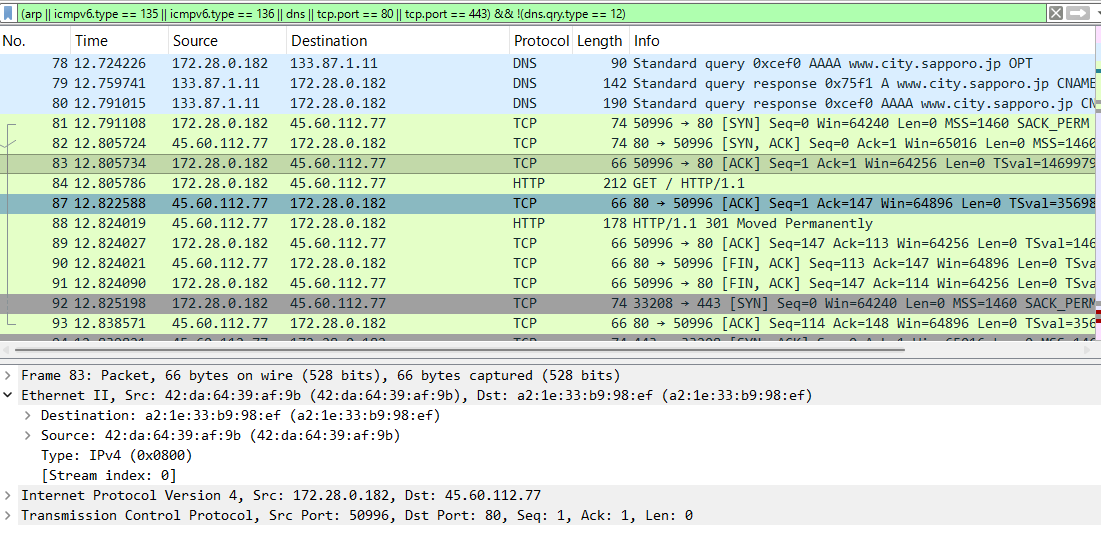
\includegraphics[width=0.98\columnwidth]{fig/wireshark_e_sapporo.png}
    \caption{www.city.sapporo.jpへのアクセスをWiresharkで読み取った結果}
    \label{fig:ws_e_sapporo}
  \end{figure}

  \begin{figure}[h]
    \centering
    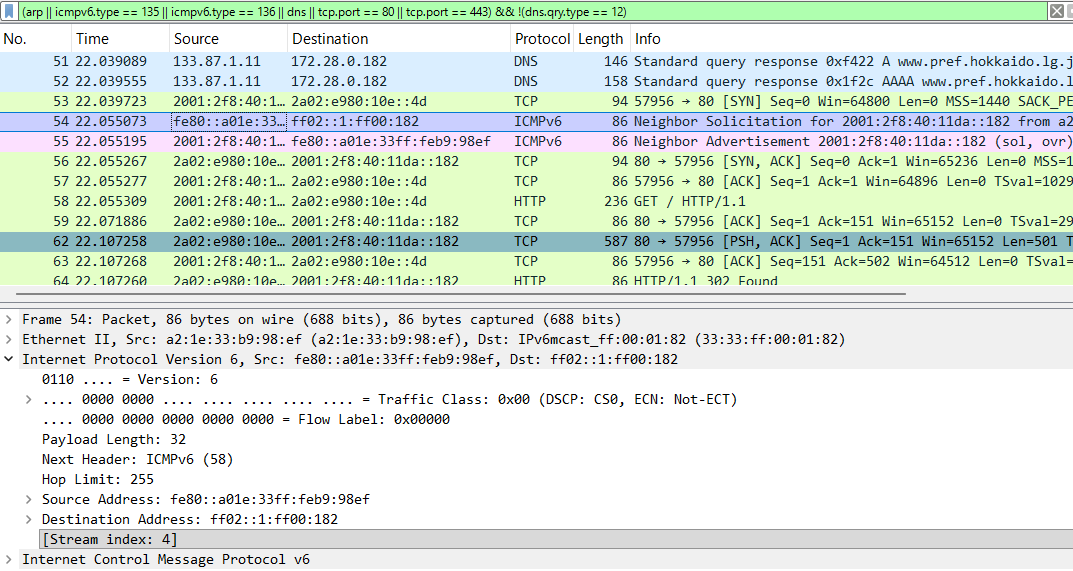
\includegraphics[width=0.98\columnwidth]{fig/wireshark_e_hokkaido.png}
    \caption{www.pref.hokkaido.lg.jpへのアクセスをWiresharkで読み取った結果}
    \label{fig:ws_e_hokkaido}
  \end{figure}

  \begin{figure}[h]
    \centering
    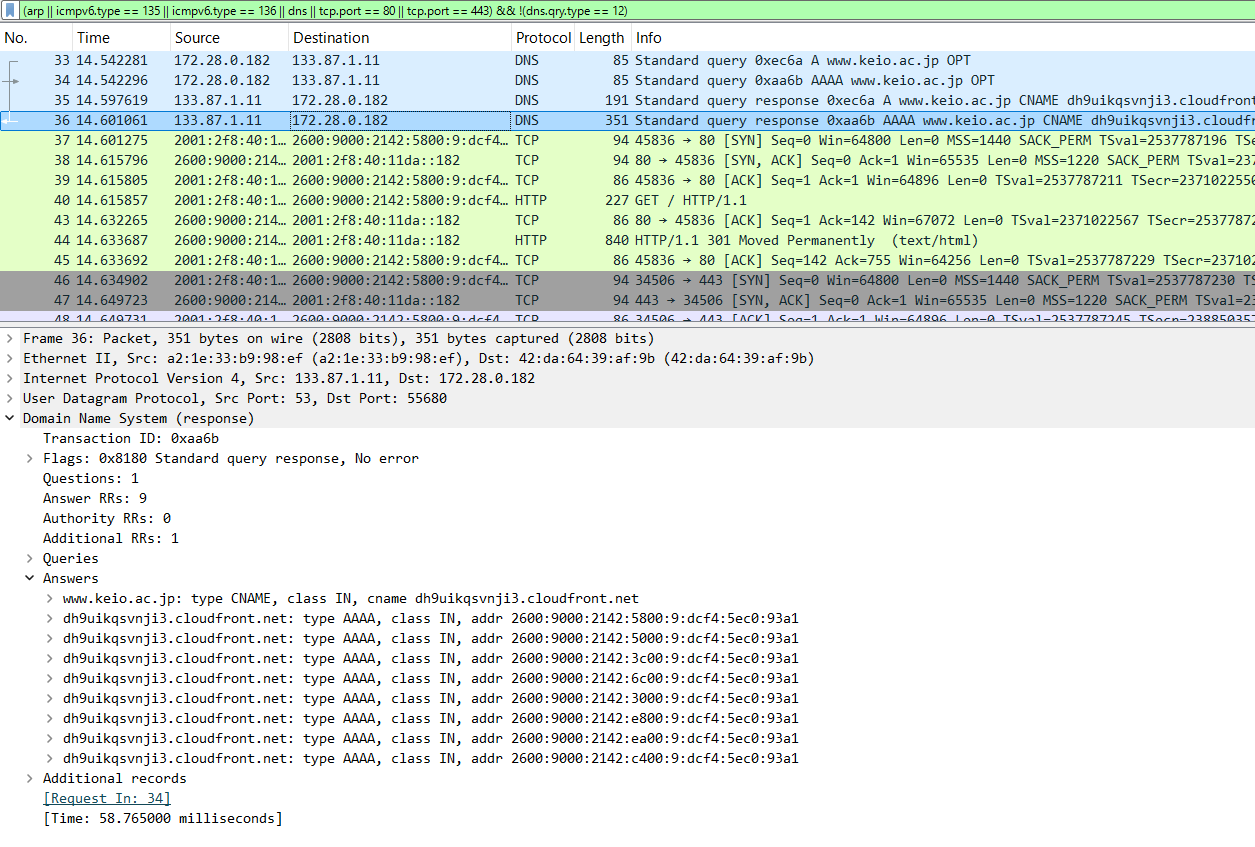
\includegraphics[width=0.98\columnwidth]{fig/wireshark_e_keio.png}
    \caption{www.keio.ac.jpへのアクセスをWiresharkで読み取った結果}
    \label{fig:ws_e_keio}
  \end{figure}

  学外への通信は，まずデフォルトゲートウェイのMACアドレスを解決することから始まる．出力\ref{out:route_e}の経路表では，デフォルトゲートウェイはIPv4が【要記入】，IPv6が【要記入】であり，近隣キャッシュには両者のMACアドレス【要記入】がすでに登録されていた．そのため，図\ref{fig:ws_e_sapporo}〜図\ref{fig:ws_e_keio}では【ARP/NDのパケットが現れなかった／現れた】．【現れなかった場合：キャッシュの内容(出力\ref{out:route_e})から，ゲートウェイのMACアドレスは既知であったと言える．】

  www.city.sapporo.jpでは，図\ref{fig:ws_e_sapporo}のNo.【要記入】で名前解決のためAレコードの問い合わせがDNSリゾルバ【要記入】に送られ，No.【要記入】の応答でアドレス【要記入】が得られた．AAAAレコードの問い合わせ(No.【要記入】)に対する応答は【アドレスなし】であり，このサイトはIPv4のみに対応していることが分かる．続いて，TCPの接続後にHTTPのGETがポート80に送られ，No.【要記入】のレスポンスは【要記入：301などのステータスコードとLocation】であった．【HTTPSへ転送されている場合：その後ポート443へ接続し，TLSハンドシェイク(Client Hello，Server Hello，Certificate等)ののちHTTPSでコンテンツが取得された．】

  www.pref.hokkaido.lg.jpは，図\ref{fig:ws_e_hokkaido}のとおりAとAAAAの双方に応答があり，IPv4/IPv6の両方に対応している．wgetが実際に使用したのは【IPv4／IPv6】で，その理由は【要記入】と考えられる．HTTPおよびHTTPSの手順は【要記入】．

  www.keio.ac.jpについては，図\ref{fig:ws_e_keio}で【要記入：問い合わせるレコード，使用したIPバージョン，HTTP/HTTPSの手順】．

  以上より，【3サイトの違い（IPバージョン，リダイレクトの有無，TLSのバージョンなど）を2〜3文でまとめる】．
\end{maintask}
